\chapter{Quantum Monte-Carlo Methods} \label{chp:methods}
\epigraph{Great quote.}{Author}
\begin{figure}[H]
	\centering
	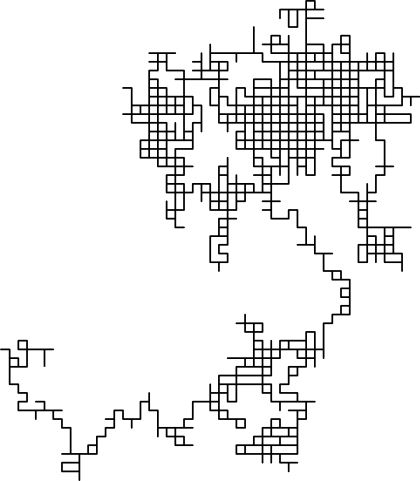
\includegraphics[scale=0.4]{Images/random_walk.png}
	\caption{Random walk in two dimensions, where the walker is restricted to move parallel to the coordinate axis.\\ © Copyright wikipedia.org.}
\end{figure}

Some great quantum many-body methods have been developed throughout the past century. The Hartree-Fock method is one of the most successful, which sets up a mean field and is thus relatively computational cheap to work with. It works also as an input to so-called post-Hartree-Fock methods, which includes configuration interaction, coupled cluster and quantum Monte-Carlo. The two former will be discussed in the next chapter, together with the Hartree-Fock method itself, and in this chapter we will dig into the quantum Monte-Carlo methods. 

Monte Carlo methods in quantum mechanics are a bunch of methods that are built on diffusion processes, and includes variational Monte Carlo (VMC), diffusion Monte Carlo (DMC) and others. The common denominator is that we move particles in order to find the optimal configuration, usually where the energy is minimized. Usually one uses the methods to study time-independent systems, but also time-dependent systems can be studied by for example time-dependent variational Monte-Carlo.

As variational Monte-Carlo is our main focus in this work, it will be explained thoroughly in this chapter together with common sampling tools. In the end, we will briefly explain the idea behind the diffusion Monte-Carlo method, as we will use the method as reference for our results. 

\section{Variational Monte-Carlo} \label{subsec:vmc}
The variational Monte-Carlo (hereafter VMC) method is today widely used when it comes to the study of ground state properties of quantum mechanical systems. It is a Markov chain Monte-Carlo method which makes use of Metropolis sampling, and has been used in studies of fermionic systems since the 1970's. \cite{deb_variational_2014} If we go back to the variational principle in equation \eqref{eq:variationalprinciple}, we see that by choosing a wave function which satisfies the criteria, we will get an energy larger or equal to the ground state energy. \bigskip

There are two main problems we need to solve
\begin{enumerate}
	\item We seldomly know the correct wave function
	\item The integral we need to find the energy is hard or impossible to solve
\end{enumerate}
Let us first determine the last problem, which often is considered as the root of all evil. Solving this integral analytically is impossible, but we can approximate it with a sum,
\begin{align}
E &\leq \frac{\int d\bs{r}\Psi_T(\bs{r})^*\hat{\mathcal{H}}\Psi_T(\bs{r})}{\int d\bs{r}\Psi_T(\bs{r})^*\Psi_T(\bs{r})} \notag\\
& = \int P(\bs{r}) E_L(\bs{r}) d\bs{r} \notag\\
& \approx \frac{1}{M}\sum_{i=1}^ME_L(\bs{r}_i) \label{eq:energysum}
\end{align}
which is a common trick in statistical physics. The local energy is defined as
\begin{equation}
E_L(\bs{r})\equiv\frac{1}{\Psi_T(\bs{r})}\hat{\mathcal{H}}\Psi_T(\bs{r})
\label{eq:local energy}
\end{equation}
and the $\bs{r}_i$ is withdrawn from the probability distribution $P(\bs{r})$, which is given by
\begin{equation}
P(\bs{r})=\frac{|\Psi_T(\bs{r})|^2}{\int d\bs{r}|\Psi_T(\bs{r})|^2}.
\label{eq:probvmc}
\end{equation}
When increasing the number of energies drawn from the distribution, $M$, henceforth denoted as Monte-Carlo cycles, the standard error decreases and we get a more accurate energy. The error goes as $\mathcal{O}(1/\sqrt{M})$, and in the limit when $M$ goes to infinity, the error goes to zero,
\begin{equation}
\langle E_L\rangle=\lim_{M\to\infty} \frac{1}{M}\sum_{i=1}^ME_L(\bs{r}_i).
\end{equation}

Zero-variance property: 
For more statistical details, see \cite{deb_variational_2014}. 

So far, so good, but how about the first problem stated above? How do we find the correct wave function? In VMC, we define a wave function with variational parameters, which are adjusted in order to minimize the energy for every iteration. Of course, we need a decent initial guess, which is usually based on our physical intuition. We will later examine how much physical intuition we need to get an acceptable result. 

For every iteration, we run $M$ Monte-Carlo cycles where we withdraw a new position $\bs{r}_i$. Whether or not the proposed move should be accepted is determined by the Metropolis algorithm.

\section{The Metropolis algorithm}
Metropolis sampling is a method of accepting or rejecting moves in Markov chains, and is today often the preferred sampling algorithm in quantum Monte-Carlo. The genius of this algorithm, is that the acceptance of a move is not based on the probabilities themselves, but the ratio between the new and the old probabilities. In that way, we avoid calculating the sum over all probabilities, which is often computational intractable. 

If we denote $\bs{r}$ as the current state, and $\bs{r}'$ as the proposed state, we have a transition rule $P(\bs{r}'|\bs{r})$ for going from $\bs{r}$ to $\bs{r}'$ and a transition rule $P(\bs{r}|\bs{r}')$ for going the other way around. If we then assume that the rules satisfy \textit{ergodicity} and \textit{detailed balance}, we have the following relationship:
\begin{equation}
P(\bs{r}'|\bs{r})P(\bs{r})=P(\bs{r}|\bs{r}')P(\bs{r}').
\end{equation}

The next step is to rewrite the transition rules in terms of a proposal distribution $T(\bs{r}'|\bs{r})$ and an acceptance probability $A(\bs{r}',\bs{r})$,
\begin{equation}
P(\bs{r}'|\bs{r})=T(\bs{r}'|\bs{r})A(\bs{r}',\bs{r}).
\end{equation}
In order to satisfy the detailed balance, we need to choose $A(\bs{r}\rightarrow\bs{r}')$ such that
\begin{equation}
A(\bs{r}',\bs{r})=\text{min }\left[1,\frac{T(\bs{r}|\bs{r}')P(\bs{r}')}{T(\bs{r}'|\bs{r})P(\bs{r})}\right],
\label{eq:acceptance}
\end{equation}
since $A$ cannot be larger than 1. If the acceptance is higher than a random number between 0 and 1, the move is accepted.

\subsection{Brute-force sampling}
In its simplest form, the move is proposed randomly both in magnitude and direction. Mathematically, we can write this as
\begin{equation}
\bs{r}'=\bs{r}+sd\bs{r}
\end{equation}
where $s$ is a random number which determines the distance to move and $d\bs{r}$ is a random direction (typically which particle to move). We obtain the naive acceptance probability when requiring $T(\bs{r}'|\bs{r})=T(\bs{r}|\bs{r}')$, such that the it simplifies to
\begin{equation}
A(\bs{r}',\bs{r})=\text{min }\left[1,\frac{P(\bs{r}')}{P(\bs{r})}\right].
\end{equation}

However, with this approach a lot of moves will be rejected, which results in a significant waste of computing power. A better method is \textbf{importance sampling}.

\subsection{Importance sampling}
Importance sampling is a more intelligent sampling method than the brute-force sampling, since the new position is based on an educated guess. To understand how it works, we need to take a quick look at diffusion processes. We start from the Fokker-Planck equation,
\begin{equation}
\frac{\partial P(\bs{r},t)}{\partial t}=D\nabla\left(\nabla-\bs{F}\right)P(\bs{r},t)
\end{equation}
which describes how a probability distribution $P(\bs{r},t)$ evolves in appearance of a drift force $\bs{F}$. In the case $\bs{F}=0$, the equation reduces to the diffusion equation with $D$ as the diffusion constant. This simplifies to $D=1/2$ in atomic units. 

The Langevin equation states that a diffusion particle tends to move parallel to the drift force in the coordinate space, but because of a random variable $\bs{\eta}$ this is not always true. The equation reads
\begin{equation}
\frac{\partial \bs{r}(t)}{\partial t}=D\bs{F}(\bs{r}(t))+\bs{\eta}.
\label{eq:langevin}
\end{equation}
Given a position $\bs{r}$, the new position $\bs{r}'$ can be be found by applying forward-Euler on equation \eqref{eq:langevin},
\begin{equation}
%\bs{r}'=\bs{r}+D\bs{F}(\bs{r})\Delta t + \bs{\xi}\sqrt{\Delta t}
\end{equation}
where $\Delta t$ is a fictive time step and $\bs{\xi}$ is a Gaussian random variable. The next thing we want to find, is an expression for the drift force $\bs{F}$ which makes the system converge to a stationary state. 

A stationary state is found when the probability density $P(\bs{r})$ is constant in time, i.e, when the left-hand-side of Fokker-Planck is zero. In that case, we can write the equation as
\begin{equation}
\nabla^2P(\bs{r})=P(\bs{r})\nabla\bs{F(\bs{r})}+\bs{F(\bs{r})}\nabla P(\bs{r}).
\end{equation}
In the next, we assume that the drift force takes the form $\bs{F(\bs{r})}=g(\bs{r})\nabla P(\bs{r})$, since the force should point to a higher probability. We can then go further and write
\begin{equation}
\nabla^2 P(\bs{r})\big(1-P(\bs{r})g(\bs{r})\big)=\nabla\big(g(\bs{r})P(\bs{r})\big)\nabla P(\bs{r})
\end{equation}
which is satisfied when $g(\bs{r})=1/P(\bs{r})$. We then get the drift force 
\begin{equation}
\bs{F}(\bs{r})=\frac{\nabla P(\bs{r})}{P(\bs{r})}=2\frac{\nabla\Psi_T(\bs{r})}{\Psi_T(\bs{r})},
\end{equation}
which is also known as the \textit{quantum force}.

The remaining part is how to decide if a proposed move should be accepted or not. For this, we need to find the sampling distributions $T(\bs{r}'|\bs{r})$ from equation \eqref{eq:acceptance}, which are just the solutions of the Fokker-Planck equation. The solutions read
\begin{equation}
G(\bs{r},\bs{r}',\Delta t)\propto\exp\Big(-\big(\bs{r}-\bs{r}'-D\Delta t\bs{F}(\bs{r})\big)^2/4D\Delta t\Big)
\end{equation}
which is called Green's functions. They correspond to the normal distribution $\mathcal{N}(\bs{r}|\bs{r}'+D\Delta t \bs{F}(\bs{r}),2D\Delta t)$. The acceptance probability for importance sampling can finally be written as
\begin{equation}
A(\bs{r}'|\bs{r})=\text{min }\left[1,\frac{G(\bs{r},\bs{r}',\Delta t)P(\bs{r}')}{G(\bs{r}',\bs{r}, \Delta t)P(\bs{r})}\right],
\end{equation}
where the marginal probabilities are still given by equation \eqref{eq:probvmc}. As a summary, we set up the actual algorithm, known as Metropolis-Hasting's algorithm, see algorithm \eqref{alg:hasting}.

\IncMargin{1em}
\begin{algorithm}
	\SetAlgoLined
	\Parameter{$\Delta t$: Fictive time step}
	\Data{$\bs{r}'$: Initial particle positions}
	\Data{$\bs{\theta}$: Initial parameters}
	\Require{$\Psi_T(\bs{r};\bs{\theta})$: Initial trial wave function guess}
	\BlankLine
	$\bs{F}(\bs{r}')\leftarrow2(\nabla\Psi_T(\bs{r}'))/\Psi_T(\bs{r}')$ (Initialize the quantum force)\;
	$G(\bs{r}',\Delta t;\bs{\theta})\leftarrow\exp(-(D\Delta t\bs{F}(\bs{r}))^2/4D\Delta t)$ (Initialize Green's function) \;
	\While{not converged}{
		$\bs{r}=\bs{r}'$\;
		$\Psi_T(\bs{r};\theta)=\Psi_T(\bs{r}';\theta)$\;
		$G(\bs{r},\bs{r}',\Delta t;\theta)=G(\bs{r}',\bs{r},\Delta t;\theta)$\;
		\BlankLine
		$\bs{r}'=\bs{r}+D\bs{F}(\bs{r;\theta})\Delta t + \bs{\xi}\sqrt{\Delta t}$\;
		$p=|\Psi_T(\bs{r}';\theta)|^2/|\Psi_T(\bs{r};\theta)|^2$\;
		$g=G(\bs{r}',\bs{r},\Delta t;\theta)/G(\bs{r},\bs{r}',\Delta t;\theta)$\;
		$w=gp$\;
		$r=\mathcal{U}(0,1)$\;
		\eIf{$w<r$}{
			$\bs{r}'=\bs{r}$\;
			$P(\bs{r}';\theta)=P(\bs{r};\theta)$\;
			$G(\bs{r}',\bs{r},\Delta t;\theta)=G(\bs{r},\bs{r}',\Delta t;\theta)$\;
		}
		{
			keep going\;
		}
	}
	\KwResult{The optimized trial wave function.}
	\caption{The Metropolis-Hastings algorithm. The positions are chosen randomly or was chosen by a previous sampling. The parameters are also usually initialized randomly or chosen by a parameter update. The diffusion constant $D=1/2$ in natural units. }
	\label{alg:hastings}
\end{algorithm}\DecMargin{1em}

\subsection{Gibbs sampling}
In the machine learning community, Gibbs sampling is widely used when it comes to training Boltzmann machines. It is an instance of the Metropolis-Hastings algorithm, but since the units are updated to maximize the probabilities, all the moves are accepted. The algorithm will be discussed for the restricted Boltzmann case only.

Given an initial set of coordinates $\bs{r}$ and $\bs{h}$, one can use the conditional probability $P(\bs{r}|\bs{h})$ to find a new set of 

\section{Diffusion Monte-Carlo}
Diffusion Monte-Carlo belongs to a class of projection and Green's function approaches. Consider the time-imaginary Schrödinger equation
\begin{eqnarray}
-\frac{\partial\Psi(\bs{r},\tau)}{\partial\tau}=(\mathcal{H}-E_T)\Psi(\bs{r},\tau)
\end{eqnarray}
where $\tau$ is the imaginary time and $E_T$ is an energy offset. 
